\synctex=1
\documentclass[11pt]{beamer}
\usepackage{microtype}
\usepackage[utf8]{inputenc}
\usepackage[french]{babel}
\uselanguage{French}
\usepackage{minted}

\usepackage{lectureb}
\usetheme{CambridgeUS}
\topic{Introduction}

\author{
  Pablo Oliveira
}

\begin{document}

\maketitle

\begin{slide}{Informations Administratives (1)}
\itms{
  \item Cours Systèmes Exploitations Avancé (SEA)
  \item Site du cours: \url{https://www.sifflez.org/lectures/SEA/}
  \ittms{
    \item Emploi du temps, documents et notes de cours
  }
  \item Bibliographie:
  \ittms{
    \item \emph{Operating System Concepts, 8th Edition}, \\
     de Silberschatz, Galvin, and Gagne
    \item \emph{Modern Operating Systems, 4th Edition}, \\
     de Tanembaum
    \item \emph{Stanford CS 140 lectures Winter'14}, \\
      de David Mazières
  }
}
\end{slide}

\begin{slide}{Informations Administratives (2)}
\itms{
  \item Prof.:  \texttt{pablo.oliveira@uvsq.fr}
  \item Group de discussion (inscription obligatoire)
    \ittms{
      \item \url{https://groups.google.com/group/iatic4-os/}
      \item Poser des questions sur les cours, TDs, projets.
      \item Tout le monde est encouragé à répondre !
    }
  \item Dates clés:
  \ittms{
    \item Cours: Vendredi 08:15-10:15 214
    \item TDs: Vendredi G1 10:30-13:00 -- G2 14:15-16:45
  }
  \item Contrôle Continu
  \ittms{
    \item 30\% Mini-Projets notés
    \item 35\% QCMs en début de cours
    \item 35\% Contrôle
  }
}
\end{slide}

\begin{slide}{Sujets abordés}
\itms{
  \item Threads et Processus
  \item Concurrence et Synchronisation
  \item Ordonnancement
  \item Mémoire virtuelle
  \item Entrées/Sorties
  \item Protection \& Securité
  \item Systèmes de Fichiers
  \item Machines Virtuelles

  \item Note:  Nous prendrons souvent Unix comme example
  \ittms{
    \item SE actuels et futurs fortement influencés par Unix
    \item Windows est l'exception
  }
}
\end{slide}

\begin{slide}{Systèmes d'Exploitation 1}
\itms{
  \item Présentation des SE du point de vue de \emph{l'utilisateur}
  \ittms{
     \item Utilisation du shell (commandes de base, redirections, tubes/pipes)
     \item Création de threads et processus
     \item Introduction à l'ordonnancement
     \item Utilisation des principaux appels systèmes
     \item Projet: sytème de fichiers virtuel
  }
}
\end{slide}

\begin{slide}{Objectifs du cours}

\itms{
  \item Présentation des SE du point de vue du \emph{concepteur}
  \item Approfondir les concepts fondamentaux des SE
  \ittms{
    \item Comprendre le SE fait de vous de meilleurs programmeurs
  }
  \item Comprendre les enjeux et l'implémentation des méchanismes des SE
  \ittms{
    \item Caching, concurrency, memory management, I/O, protection
  }
  \item Vous apprendre à travailler avec un projet logiciel complexe
  \ittms{
    \item Attention:  ce cours est considéré difficile par de nombreux étudiants
    \item TDs: beaucoup de code à rendre
    \item Travail régulier et soutenu nécessaire
  }
}
\end{slide}

\begin{slide}{Notation}

\itms{
  \item Note Finale =
  \ittms{
    \item 40\% Contrôle Continu
    \item 30\% QCM
    \item 30\% TDs
    }
}
\end{slide}

\begin{slide}{TDs}
\itms{
  \item Ne pas utiliser/récupérer les solutions des autres groupes
  \ittms{
    \item Vos rendus sont comparés avec un logiciel anti-plagiat
    \item Ne publiez pas vos solutions
    \item Respectez la charte anti-plagiat de l'UVSQ (document disponible
      sur le portail de l'ISTY)
  }
  \item \Red{Citez tout code dont vous vous inspirez}
  \ittms{
    \item Si c'est cité, c'est pas de la triche
    \item Des points seront déduits si une grosse partie rendu est
      du code extérieur. Mais les emprunts cités n'entrainerons pas de sanctions.
  }
}
\end{slide}

\begin{slide}{Qu'est ce qu'un système d'exploitation ?}
\itms{
\item Interface entre les applications et le materiel \\
\centerline{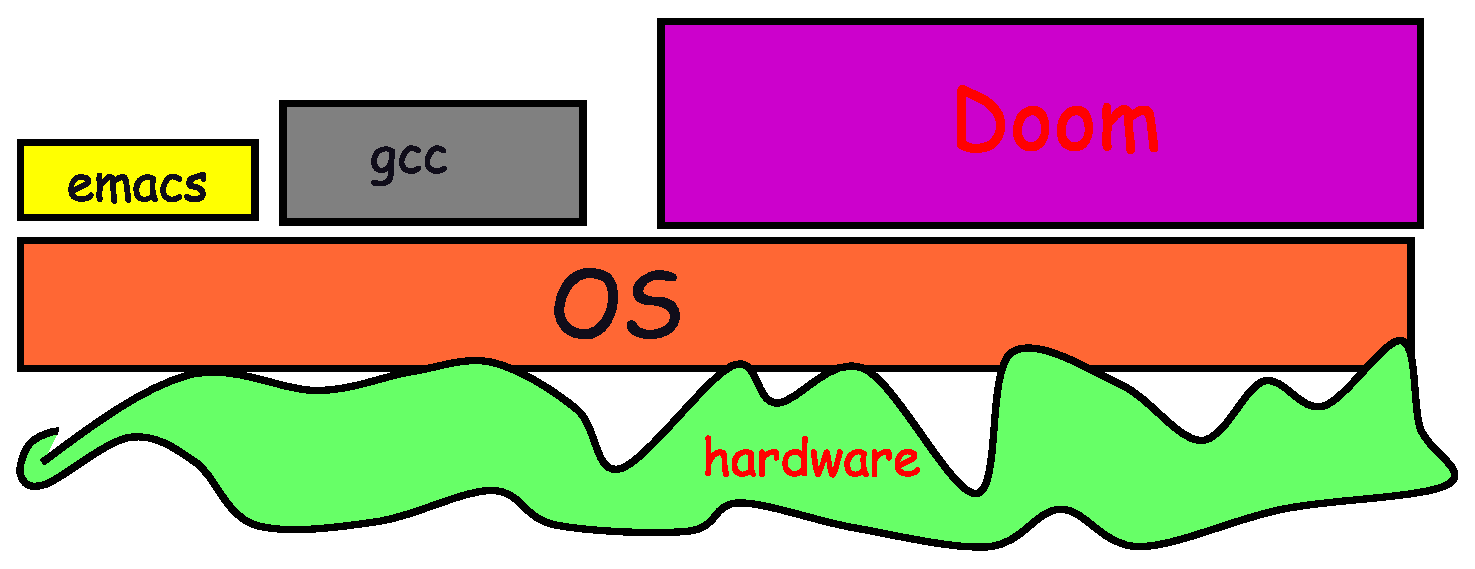
\includegraphics[width=3in]{figs/whatis}}
 \item Rends le matériel utilisable par le programmeur
 \item{} [Souvent] Abstrait le matériel
  \ittms{
   \item Gère et cache les détails du matériel
   \item Accède au matériel à travers des interfaces bas niveau interdites aux applications  }
 \item{} [Parfois] Protège
  \ittms{
   \item Evite qu'un utilisateur/processus puisse lire/détruire les données d'un autre utilisateur/processus
  }
}
\end{slide}

\begin{slide}{Pourquoi étudier les systèmes d'exploitation ?}
\itms{
  \item Concepts système importants pour bien programmer la machine
  \ittms{
    \item Important pour HPC ou applications critiques
    \item Algorithmes réutilisables dans d'autres contextes
    \item Important pour comprendre l'intéraction avec le matériel
  }
  \item Comprendre les Serveurs Haute Performance
  \ittms{
    \item Mêmes problèmes que dans un SE
  }
  \item Comprendre le Partage des Resources
  \ittms{
    \item Durée de la batterie, spectre Hertzien, etc.
  }
  \item Comprendre la Sécurité
  \ittms{
    \item Isolation, capabilités, DoS, etc.
  }
  \item Apparition de nouveaux SE embarqués (eg. Android)
  \item Navigateur ressemble de plus en plus à un SE (eg. Chrome isolation des tabs)
}
\end{slide}

\begin{frame}{Années 40-50: Super calculateur ENIAC}

\centering
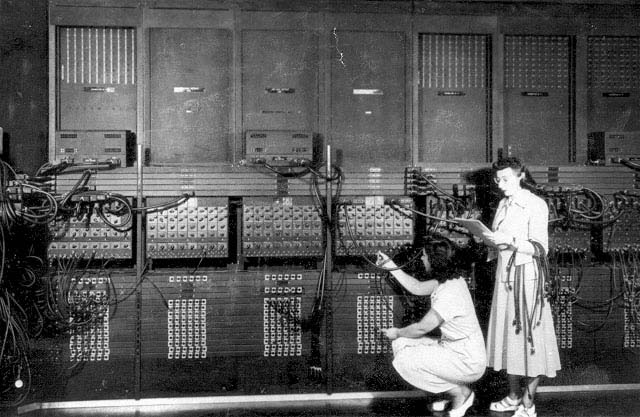
\includegraphics[width=0.95\textwidth]{figs/eniac.jpg}
\end{frame}


\begin{frame}{Années 40-50: Super calculateur ENIAC}

\begin{itemize}
\itemsep1pt\parskip0pt\parsep0pt
\item
  1946: P. Eckert et J. Mauchly, simulation des tirs d'artillerie

  \begin{itemize}
  \itemsep1pt\parskip0pt\parsep0pt
  \item
    fréquence 100kHz
  \item
    Turing-complet
  \item
    Programmable avec des interrupteurs et tableau de connexion
  \end{itemize}
\end{itemize}
\end{frame}

\begin{frame}{Système Exploitation des premiers Calculateurs ?}

\begin{itemize}
\itemsep1pt\parskip0pt\parsep0pt
\item
  Calculateurs gigantesques:

  \begin{itemize}
  \itemsep1pt\parskip0pt\parsep0pt
  \item
    Dizaines de milliers de relais mécaniques
  \item
    Remplacés par des lampes
  \end{itemize}
\item
  Programmation:
  \begin{itemize}
  \item
    Manuelle
  \item
    En langage machine avec des panneaux de connexion
  \item
    Pas de SE, le programme tourne directement sur la machine
  \item
    1950: généralisation des cartes perforées
  \end{itemize}
\end{itemize}
\end{frame}

\begin{frame}{IBM 701}
  \centering
  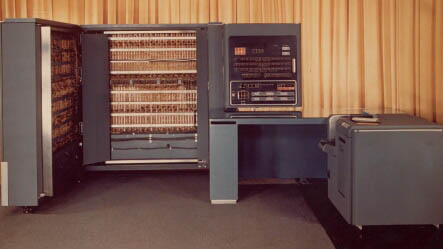
\includegraphics[width=0.95\textwidth]{figs/ibm701.png}
\end{frame}

\begin{frame}{Traitements par lots (55-65)}
\begin{itemize}
\item
  Invention des transistors en silicone (1954):

  \begin{itemize}
  \item
    plus petit et rapide que les lampes
  \item
    Bell Labs TRADIC (1MHz) et IBM 608
  \end{itemize}
\item
  Opérateurs:

  \begin{itemize}
  \itemsep1pt\parskip0pt\parsep0pt
  \item
    Chargés de la surveillance du système
  \item
    Allocation et supervision des tâches
  \end{itemize}
\item
  Les tâches sont traitées par lots:
  \begin{itemize}
      \item Des opérateurs chargent les cartes perforées pour chaque programme
  \end{itemize}
\end{itemize}
\end{frame}


\begin{frame}{Moniteur Résident}
  \begin{itemize}
  \itemsep1pt\parskip0pt\parsep0pt
  \item
    Bandes magnétiques remplacent les cartes perforées
  \item
    Moniteur résident: premier SE

    \begin{itemize}
    \itemsep1pt\parskip0pt\parsep0pt
    \item
      Il charge automatiquement les tâches successivement
      \texttt{\$LOAD} et \texttt{\$RUN}
    \item Problème : inactivité du CPU pendant les chargements depuis la bande.
    \end{itemize}
  \end{itemize}
\end{frame}

\begin{slide}{Systèmes d'Exploitation Primitifs}
\itms{
\item Juste une librairie de services standards [pas de protection]
  \ittms{
    \item[] 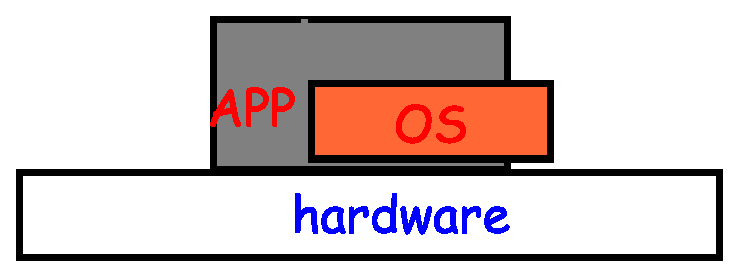
\includegraphics[width=2.5in]{figs/os0}
    \item Interface standard communique avec des pilotes matériels
  }
  \item Hypothèses simplificatrices
  \ittms{
    \item Un seul programme tourne à la fois
    \item Pas de programmes ou utilisateurs malicieux (mauvaise hypothèse)
  }
  \item Problème: Mauvaise utilisation des ressources
  \ittms{
  \item \ldots du matériel (e.g., CPU attends que le disque envoie les données)
    \item \ldots de l'humain (doit attendre la fin d'un programme pour en lancer un nouveau)
  }
}
\end{slide}

\begin{frame}
\frametitle{Execution multi-tâche}
\centerline{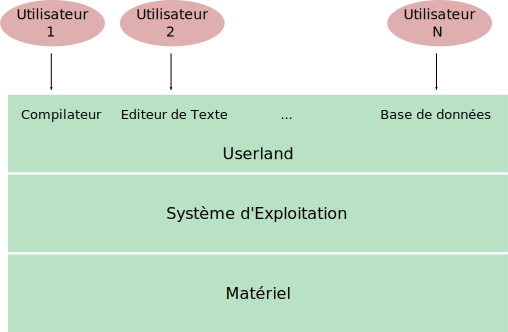
\includegraphics[width=2in]{figs/os1}}
\itms{
  \item Idée: Executer plusieurs processus en "même temps"
  \ittms{
  \item Lorsque un processus bloque (attente disque, réseau, entrée clavier, etc.)
        on execute un autre processus
  }
  \item Problème: Que peut faire un processus malicieux/mal écrit ?
\pause
  \ittms{
    \item Boucle infinie et ne jamais lâcher le CPU
    \item Écraser la mémoire d'autres processus pour les faire cracher
  }
  \item SE propose des mécanismes pour empêcher ces problèmes
  \ittms{
    \item \emph{Préemption} -- interrompt régulièrement le processus boucle infinie
    \item \emph{Protection mémoire} -- Chaque processus ne peut écrire que sur sa propre mémoire
  }
}
\end{frame}

\begin{slide}{SE Multi Utilisateurs}
  \centerline{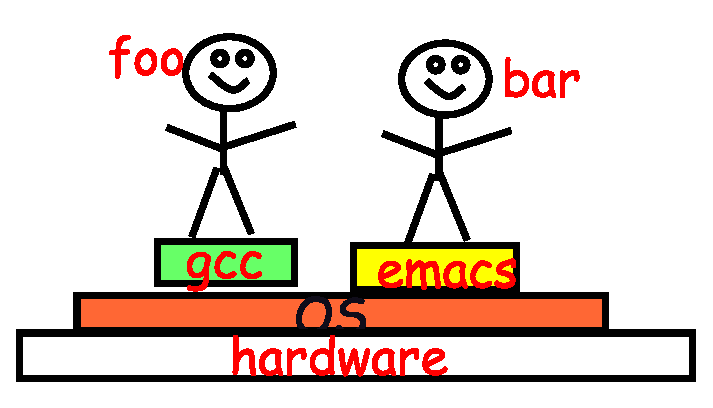
\includegraphics[height=1.3in]{figs/os2}}
  \itms{
  \item Idée:  Avec $N$ utilisateurs, système n'est pas forcément $N$ fois plus lent
    \ittms{
    \item Les demandes de CPU, mémoire, etc. sont intermittentes
    \item Tous les programmes n'ont pas besoin de la même ressource simultanément
    }
  \item Où ça peut coincer ?
    \pause
    \ittms{
    \item Utilisateurs gloutons (mise en place de politiques d'allocation)
    \item Mémoire utilisée par l'ensemble des processus supérieure à la mémoire disponible (virtualisation)
    \item Ralentissements super-linéaire (trashing)
    }
  \item Les SE mettent en place des \emph{protections} pour eliminer ces problèmes
  }
\end{slide}

\begin{slide}{Protection}
\itms{
\item Mécanismes pour isoler les utilisateurs/processus malicieux
\item Préemption:
\ittms{
\item Donner une ressource, mais la reprendre au bout d'un certain temps
}
\item Médiation:
\ittms{
  \item SE est le médiateur entre les processus et les ressources
  \item Controle toutes les ressources qu'une application peut utiliser (table de capabilités)
  \item Pour chaque demande le SE vérifie que l'application à le droit de faire cette demande
}
\item Mode privilégié dans le CPU
\ittms{
  \item Applications tournent en \emph{mode utilisateur}
  \item SE tourne en \emph{mode privilégié} (ou mode noyau)
  \item Les opérations de protection ne sont disponibles qu'en \emph{node privilégié} (par exemple editer la table de capabilités).
}
}
\end{slide}

\begin{frame}
\frametitle{Structure d'un SE typique}
\centerline{\input{os}}
\itms{
  \item Les applications tournent en mode utilisateur (P[1-4])
  \item Le noyau tourne en mode privilégié \Red{[en grisé]}
  \ittms{
    \item Crée et détruit les processus
    \item Décide et vérifie qui accède au matériel
  }
}
\end{frame}

\begin{slide}{Appel Système}
\centerline{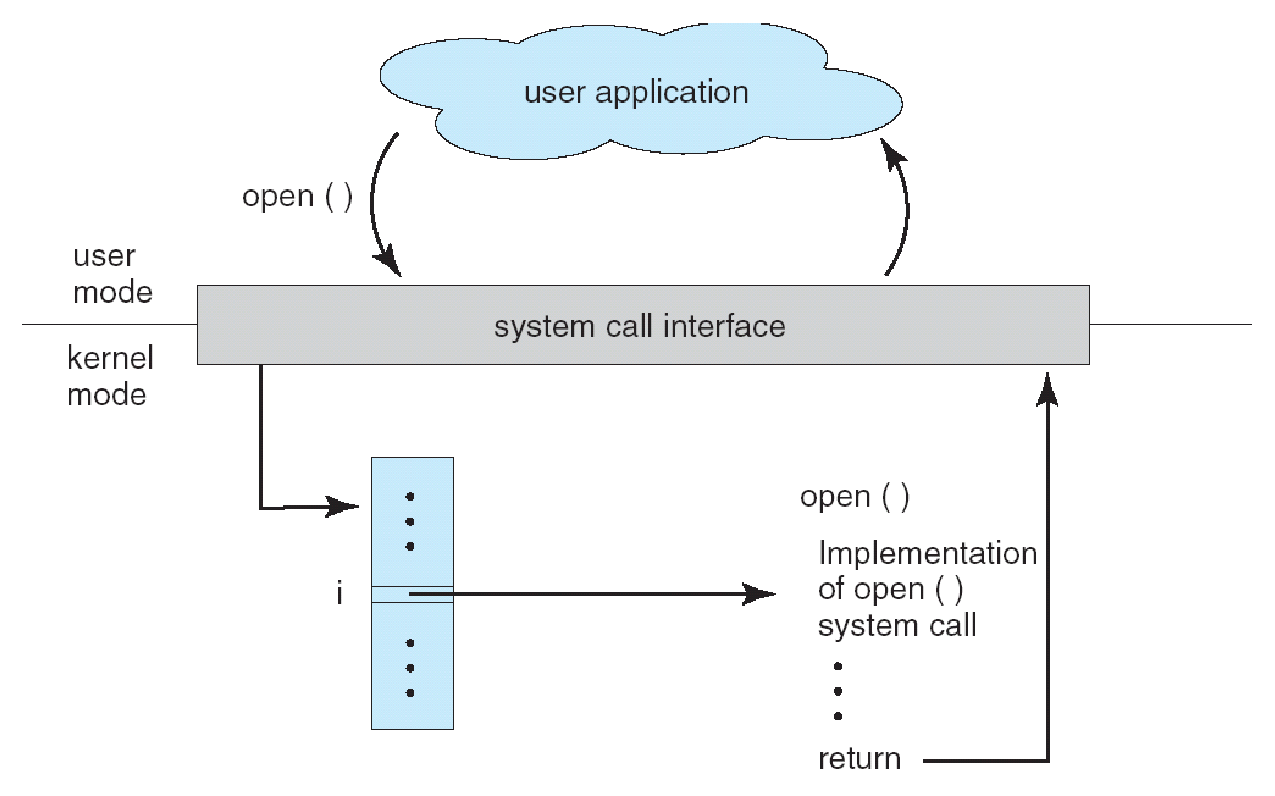
\includegraphics[height=2.3in]{figs/syscall}}
\itms{
\item Les applications invoquent le noyau avec des \emph{appels système}
  \ittms{
  \item Des instructions assembleur spéciales transfèrent le contrôle au noyau
  \item \ldots qui transfère l'appel à l'une des 100+ routines gestionnaires
  }
}
\end{slide}

\begin{slide}{Appel Système (suite)}
\itms{
  \item Objectifs: Faire des choses que l'application ne peut pas faire en mode utilisateur
  \ittms{
    \item Semblable à un appel de bibliothèque mais en mode privilégié
  }
  \item Noyau expose une interface d'appels systèmes bien définie
  \ittms{
  \item L'application configure les arguments de l'appel et appellent une "trappe" (ou interruption logicielle)
    \item Le noyau répond à la demande et retourne le résultat
  }
  \item Exemple: interface POSIX/UNIX sont des appels systèmes
  \ittms{
    \item \texttt{open, close, read, write, \ldots}
  }
  \item Fonctions de plus haut niveau sont implémentées à l'aide d'appels système
  \ittms{
    \item \texttt{printf, scanf, gets,} etc.
  }
}
\end{slide}

\begin{frame}{Mode privilégié}

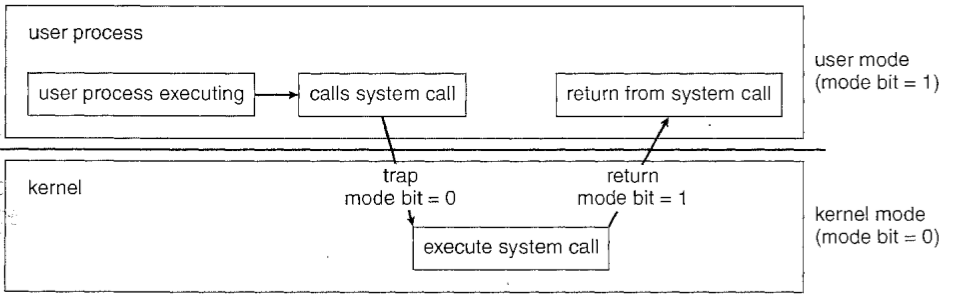
\includegraphics[width=\textwidth]{figs/dualmode.png}

\end{frame}

\begin{slide}{Exemple d'un appel système}
\centerline{\includegraphics[height=2.2in]{figs/libc}}
\itms{
  \item Librairie standard implémentée à l'aide d'appels systèmes
  \ittms{
    \item \emph{printf} -- dans la libc, mêmes privilèges que l'utilisateur
    \item appelle \emph{write} -- dans le noyau, qui peut écrire sur le disque dur, ou envoyer des bits sur les ports de sortie  }
}
\end{slide}

\begin{slide}{UNIX appels système pour les Entrées/Sorties}
\itms{
\item Les applications ouvrent des fichiers (ou des périphériques)
  \ittms{
  \item Les E/S opèrent sur des descripteurs de fichiers (des entiers)
  }
  \item \texttt{int open(char *path, int flags, /*mode*/...);}
  \ittms{
    \item \texttt{flags}: \texttt{O\_RDONLY}, \texttt{O\_WRONLY},
	\texttt{O\_RDWR}
    \item \texttt{O\_CREAT}: crée le fichier s'il n'existe pas
    \item \texttt{O\_TRUNC}: tronque le fichier
    \item \texttt{O\_APPEND}: ouvre le fichier et positionne le curseur d'écriture en fin de fichier
    \item \texttt{mode}: avec \texttt{O\_CREAT} donne les permissions du fichier
  }
  \item Retourne un descripteur de fichier
}
\end{slide}

\begin{slide}{En cas d'erreur ?}
\itms{
  \item Que se passe t'il si \texttt{open} rencontre une erreur ?
  \item La majorité des appels systèmes retournent -1 en cas d'erreur
  \ittms{
    \item L'erreur spécifique est renseignée dans la variable globale int \texttt{errno}
  }
  \item \texttt{\#include <sys/errno.h>} contient la liste des codes possibles
  \ittms{
    \item 2 = \texttt{ENOENT} ``No such file or directory''
    \item 13 = \texttt{EACCES} ``Permission Denied''
  }
  \item \texttt{perror} permet d'afficher un message adapté
  \ittms{
    \item \texttt{perror ("initfile");} \\
	$\to$ ``\texttt{initfile:\ No such file or directory}''
  }
}
\end{slide}

\begin{slide}{Operations sur des descripteurs de fichier}
\itms{
  \item \texttt{int read (int fd, void *buf, int nbytes);}
  \ittms{
    \item Retourne le nombre d'octets lus
    \item Retourne 0 lorsque la fin du fichier (EOF) est atteinte et -1 en cas d'erreur
  }
  \item \texttt{int write (int fd, void *buf, int nbytes);}
  \ittms{
    \item Retourne le nombre d'octets écrits, -1 en cas d'erreur
  }
  \item \texttt{off\_t lseek (int fd, off\_t pos, int whence);}
  \ittms{
    \item \texttt{whence}: relatif au 0 -- début, 1 -- courant, 2 -- fin
     \ittms{
       \item Retourne la position précédente dans le fichier, et -1 en cas d' error
     }
  }
  \item \texttt{int close (int fd);}
}
\end{slide}

\begin{slide}{Numéros de descripteurs de fichiers}
\itms{
  \item Les descripteurs de fichiers sont propres à un processus
  \ittms{
    \item ... mais ils sont hérités par ses fils
    \item Quand un processus crée un processus fils, ils se partagents des descripteurs
  }
  \item Les descripteurs 0, 1, et~2 ont un sens special
  \ittms{
  \item 0 -- ``entree standard'' (\texttt{stdin} ANSI C)
  \item 1 -- ``sortie standard'' (\texttt{stdout} ANSI C)
  \item 2 -- ``erreur standard'' (\texttt{stderr} ANSI C)
  \item Normalements ils sont rattachés à un terminal
  }
  \item Exemple:  \texttt{cat.c}
  \ittms{
    \item Ecrit le contenu d'un fichier sur \texttt{stdout}
  }
}
\end{slide}

\begin{slide}{\texttt{cat.c}}
  \small
  \begin{minted}{c}
     void
     typefile (char *filename)
     {
       int fd, nread;
       char buf[1024];

       fd = open (filename, O_RDONLY);
       if (fd == -1) {
         perror (filename);
         return;
       }

       while ((nread = read (fd, buf, sizeof (buf))) > 0)
         write (1, buf, nread);

       close (fd);
     }
\end{minted}
\end{slide}

\begin{frame}{Traitement des interruptions}

\begin{itemize}
\itemsep1pt\parskip0pt\parsep0pt
\item
  Une interruption suspend la tâche en cours.
\item
  Chaque interruption est associée à une routine de traitement
\item
  Un vecteur d'interruption situé à un endroit fixe en mémoire contient
  les adresses de chaque routine
\item
  On exécute la routine de traitement de l'interruption, puis on revient
  au traitement précédent.
\item
  Les routines doivent sauvegarder l'état du processeur et l'adresse du
  traitement interrompu.
\end{itemize}

\end{frame}

\begin{frame}{Deux interruptions en même temps ?}

\begin{itemize}
\itemsep1pt\parskip0pt\parsep0pt
\item
  Masquage simple

  \begin{itemize}
  \itemsep1pt\parskip0pt\parsep0pt
  \item
    Le traitement des interruptions est différé jusqu'à la fin du
    traîtement de l'interruption en cours.
  \end{itemize}
\item
  Masquage sélectif

  \begin{itemize}
  \itemsep1pt\parskip0pt\parsep0pt
  \item
    Les interruptions ont des niveaux de priorité.
  \item
    Les interruptions les plus prioritaires peuvent interrompre celles
    de niveau inférieur.
  \end{itemize}
\end{itemize}

\end{frame}

\begin{frame}{Exemple de communication périphérique}

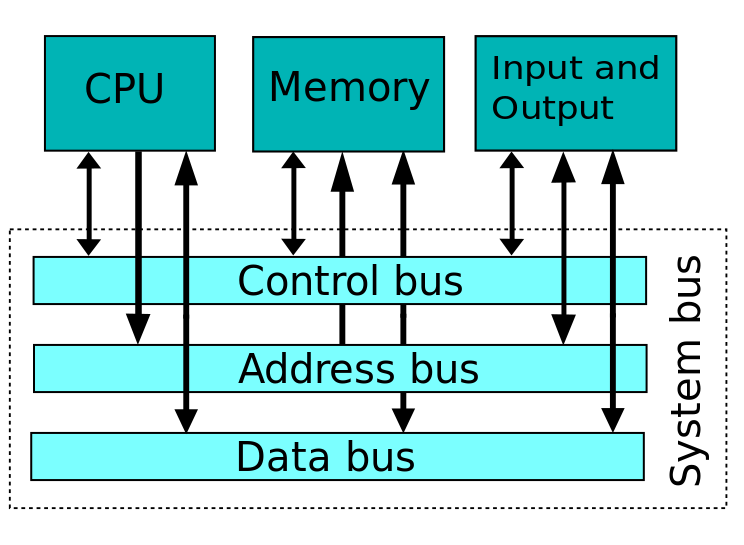
\includegraphics[width=0.4\textwidth]{figs/bus.png}

\begin{enumerate}
\def\labelenumi{\arabic{enumi}.}
\itemsep1pt\parskip0pt\parsep0pt
\item
  Le CPU écrit sur la ligne d'\emph{adresse}, la position du disque à
  lire
\item
  Le CPU active la ligne de \emph{controle} pour signaler au contrôleur
  disque
\item
  Le contrôleur disque écrit le contenu de la position demandée sur la
  ligne de \emph{données}
\item
  Il signale avec une interruption que les données sont prêtes
\end{enumerate}

\begin{itemize}
\itemsep1pt\parskip0pt\parsep0pt
\item
  Inefficace pour des gros transferts
\end{itemize}

\end{frame}



\begin{slide}{Différents contextes d'exécution}
\itms{
  \item Le système se trouve habituellement dans un des contextes suivants
  \item \emph{Processus Utilisateur:} execution d'une application en mode utilisateur
  \item \emph{Processus Noyau}:
  \ittms{
    \item Execution de code noyau à la demande d'une application
    \item eg. traîtement d'un appel système
    \item Exception (segmentation fault, division par zéro, etc.)
    \item Execution d'un processus noyau (serveur de fichiers nfs)
  }
\item \emph{Code noyau hors processus}
  \ittms{
    \item Interruption d'horloge
    \item Interruption matérielle
    \item Interruption logicielle, ``Tasklets'' (dans linux)
  }
  \item Changement de Contexte -- Changer les espaces d'adresse
  \item En attente (Idle) -- rien à faire (souvent on "éteint" ou "ralentit" le CPU)
}
\end{slide}

\begin{slide}{Mécanismes de changement de contexte}
\itms{
  \item Utilisateur $\to$ Processus Noyau:  {appel système, exception}
  \item Processus Noyau $\to$ Utilisateur/Changement Contexte:  {return}
  \item Processus Noyau $\to$ Changement Contexte:  {sleep}
  \item * $\to$ Gestionnaire d'interruption matérielle:  {IRQ matériel}
  \item Changement de Contexte $\to$ Processus Utilisateur/Noyau
}
\end{slide}

\begin{slide}{Préemption CPU}
\itms{
  \item Éviter la monopolization du CPU
  \item E.g., un timer noyau reprends la main tous les 10 ms
  \ittms{
    \item Interruption matérielle d'horloge
    \item Nécessite le mode privilégié pour reprogrammer l'horloge hardware
  }
  \item Le gestionnaire d'interruption du noyau
  \ittms{
    \item Prends le contrôle quand l'interruption d'horloge se déclenche
    \item Si d'autres processus sont en attente du CPU, il leurs donne la main
    \item Protection: mode privilégié nécessaire pour definir l'adresse du gestionnaire
    \item L'utilisateur ne peux pas "hacker" la routine de traîtement
  }
  \item Resultat: un processus malicieux ne peux pas affamer tous les autres
  \ittms{
    \item Pire cas: tout le monde aura $1/N$ du CPU si $N$ processus CPU-gloutons
  }
}
\end{slide}

\begin{slide}{Protection != Securité}
\itms{
  \item Comment monopoliser le CPU quand même ?
\pause
  \item Utiliser plusieurs processus: Fork bomb
  \item Jusqu'à encore récemment, le code suivant "met à genoux" plusieurs SE
  \ittms{
    \item[] \texttt{int main() \char`\{\ while(1) fork();\char`\}}
    \item Crée des processus jusqu'à épuisement des ressources
  }
  \item Utiliser toute la mémoire: Malloc bomb
  \item Résolu par une combinaison de technique + social
  \ittms{
  \item Solution technique: limiter les processus par utilisateur (ulimit, )
  \item Solution technique: limiter le débit de création (grsec)
  \item Social: Rebooter et crier sur les utilisateurs embêtants :-)
  \item La bonne solution dépend de l'usage
  \item Serveur de la NSA vs. Serveur Imprimante dans une PME
  }
}
\end{slide}

\begin{frame}{Allocation et Protection de la mémoire}

\begin{itemize}
\itemsep1pt\parskip0pt\parsep0pt
\item
  Le noyau alloue la mémoire
\item
  Éviter qu'une tâche utilisateur détruise les données d'une autre tâche

  \begin{itemize}
  \itemsep1pt\parskip0pt\parsep0pt
  \item
    Protection mémoire
  \end{itemize}
\item
  Gérer efficacement la mémoire:

  \begin{itemize}
  \itemsep1pt\parskip0pt\parsep0pt
  \item
    Si la RAM est pleine, le SE va déplacer la mémoire de certains
    processus sur un stockage secondaire (disque)
  \item
    swap
  \end{itemize}
\end{itemize}

\end{frame}


\begin{slide}{Protection Mémoire (1/2)}
\itms{
  \item Comment éviter que les processus écrivent dans la mémoire d'autres processus

  \item Idée Mémoire Virtuelle: Chaque processus ne voit que sa mémoire à lui.

    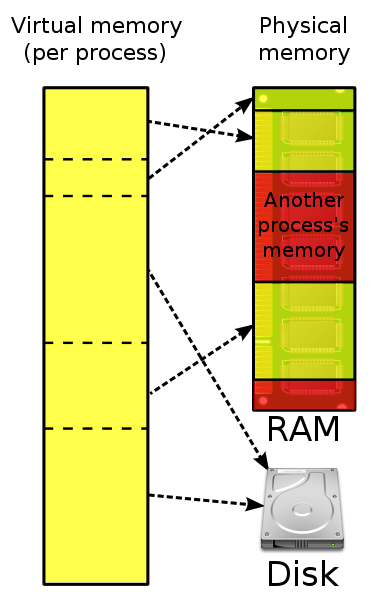
\includegraphics[height=4cm]{figs/Virtual_memory.png}
}
\end{slide}


\begin{slide}{Protection Mémoire (2/2)}
  \itms{
  \item Le CPU traduit les adresses virtuelles en adresse physiques
      en utilisant des tables de traduction à chaque accès.
  \item La table de traduction est changée à chaque changement de contexte
  \item Elle ne contient que des traductions vers des adresses autorisées

  \item Le SE peut marquer comme invalides certaines adresses virtuelles
  \ittms{
    \item Détecter les fautes de segmentation et interrompre les programmes
    \item Allocation paresseuse + SWAP \\
      (e.g., ramener les pages du SWAP uniquement lorsqu'elles sont accédées)
  }
  \item Le SE peut marquer certaines adressses comme lecture seule
    \ittms{
    \item Partage de données entre processus (par exemple le code executable de la libc)
    \item De nombreuses autres optimizations (copy on write par exemple)
  }
  \item Le SE peut marquer certaines adresses comme non exécutables
  \ittms{
    \item Rends difficile les attaques par injection de code
  }
}
\end{slide}

\begin{frame}{Temps partagé (premier vrai SE)}

\begin{itemize}
\item
  1961 CTSS (Compatible Time Sharing System)

  \begin{itemize}
  \itemsep1pt\parskip0pt\parsep0pt
  \item
    Plusieurs utilisateurs en simultané
  \item
    Ordonnanceur de tâches avec priorité
  \item
    Mémoire segmentée: sépare SE et userland
  \item
    Interrupteur d'horloge pour interrompre les tâches
  \end{itemize}
\item
  Suivi de MULTICS (Multiplexed Information and Computing System)
\item
  IBM 7094 \centering
  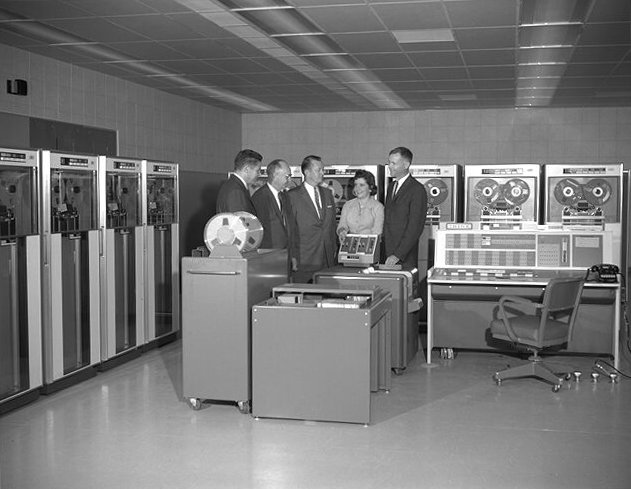
\includegraphics[width=0.5\textwidth]{figs/IBM7094.jpg}
\end{itemize}

\end{frame}

\begin{frame}{Developpement des SE}

\begin{itemize}
\itemsep1pt\parskip0pt\parsep0pt
\item
  Ken Thompson adapte MULTICS sur un PDP-7 (mini-ordinateur),
\item
  1969: ce travail devient UNIX (Bell Labs), qui donnera naissance à
  SYSTEM V et BSD
\item
  1981: Bill Gates écrit MS-DOS (Microsoft Disk Operating System)

  \begin{itemize}
  \itemsep1pt\parskip0pt\parsep0pt
  \item
    Modification du DOS de Seattle Computer Products
  \end{itemize}
\item
  1987: Tanembaum écrit MINIX (SE micro-noyau) qui servira d'inspiration
  à Linux
\item
  1991: Torvalds libère la première version de Linux
\end{itemize}

\end{frame}

\begin{frame}{Famille Unix}
\centering
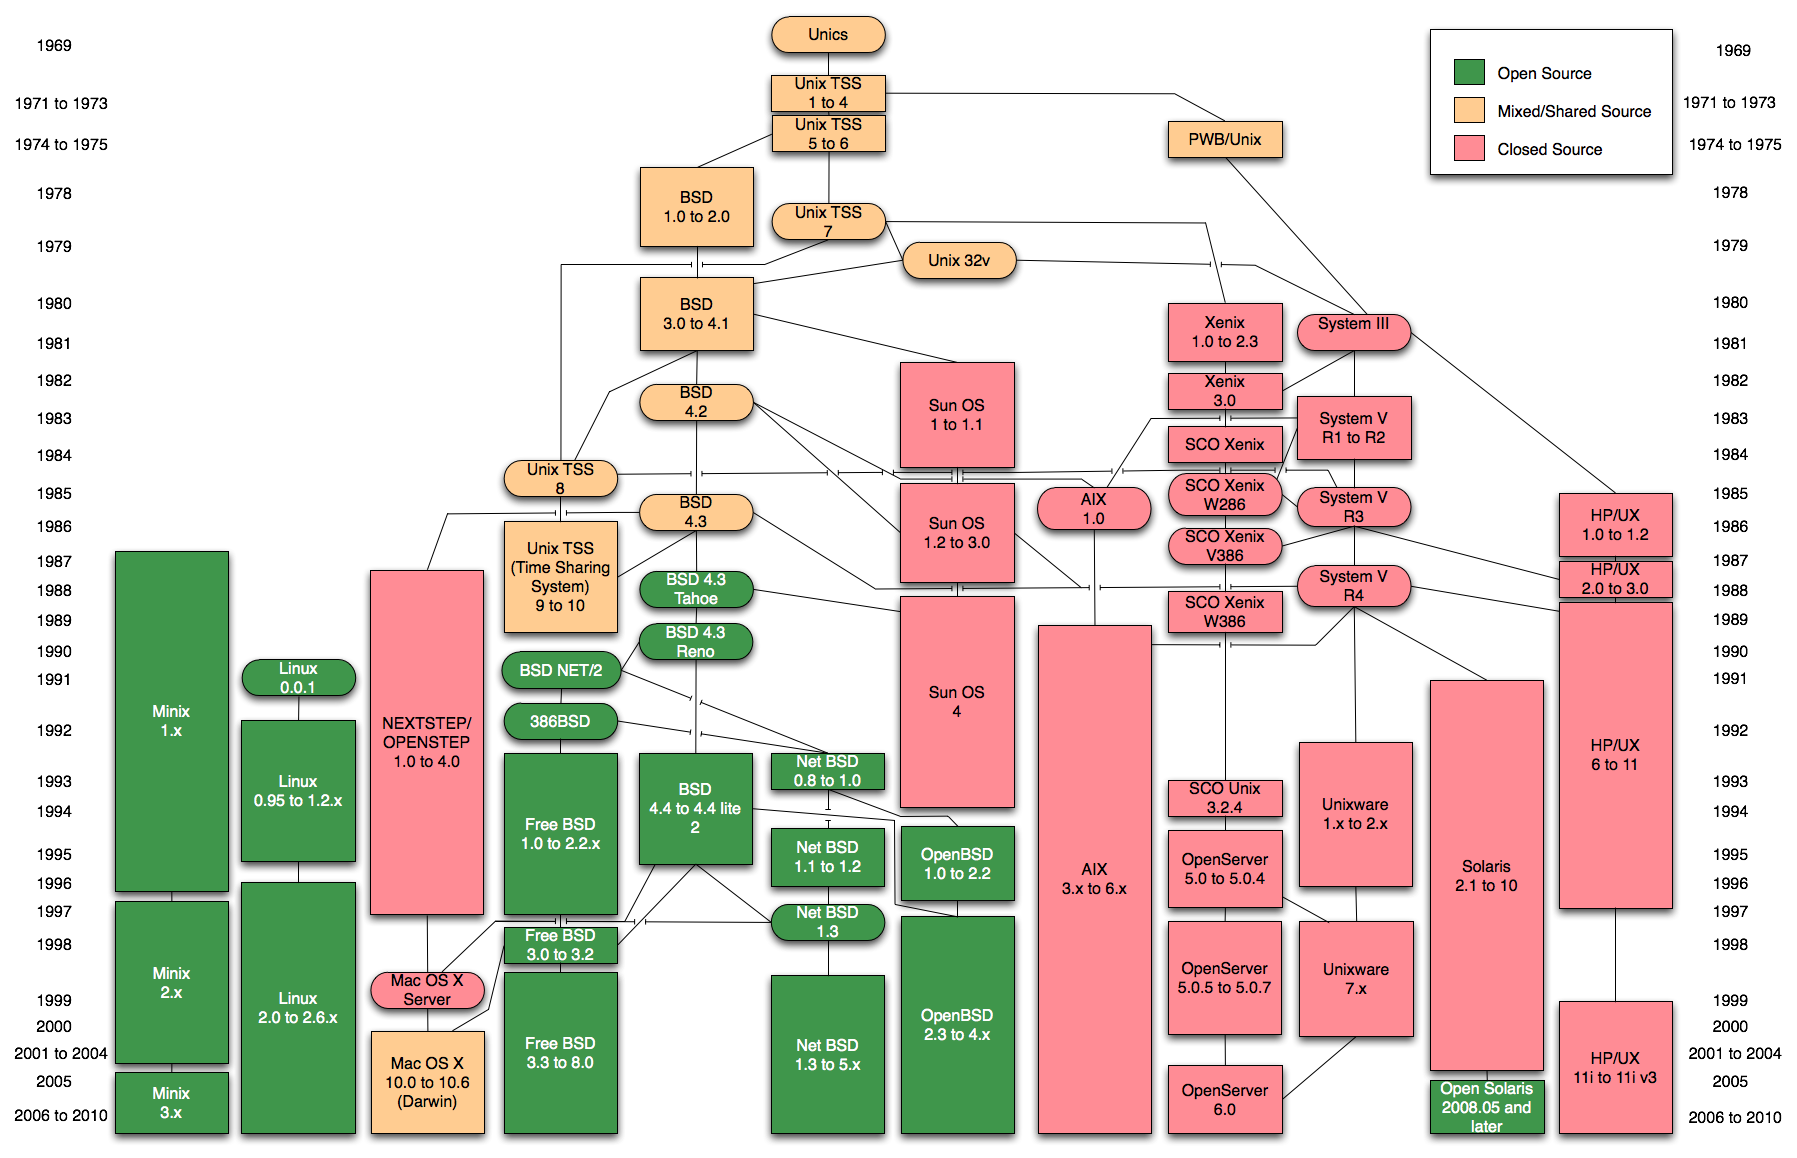
\includegraphics[width=\textwidth]{figs/unix.png}
\end{frame}

\begin{frame}{Quelques captures d'écran "vintage"}
  \centering
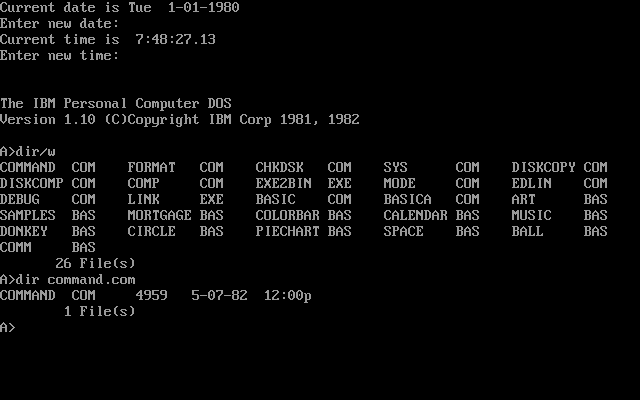
\includegraphics[width=0.4\textwidth]{figs/DOS.png}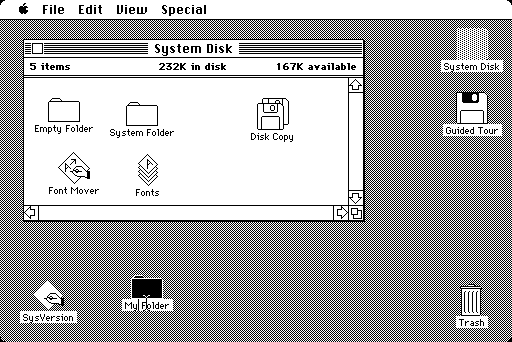
\includegraphics[width=0.4\textwidth]{figs/mac.png}

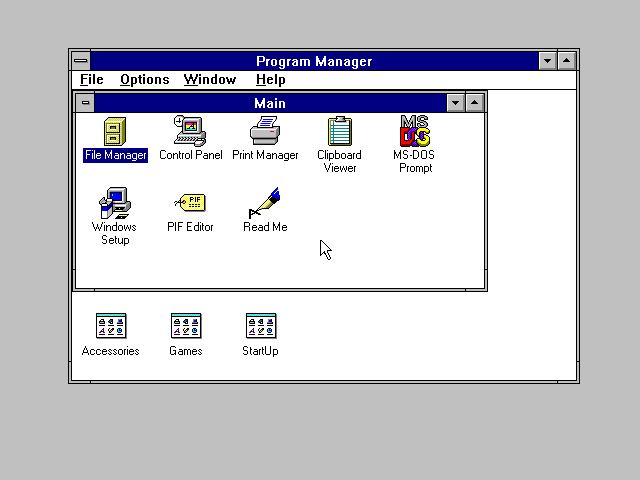
\includegraphics[width=0.4\textwidth]{figs/win31.png}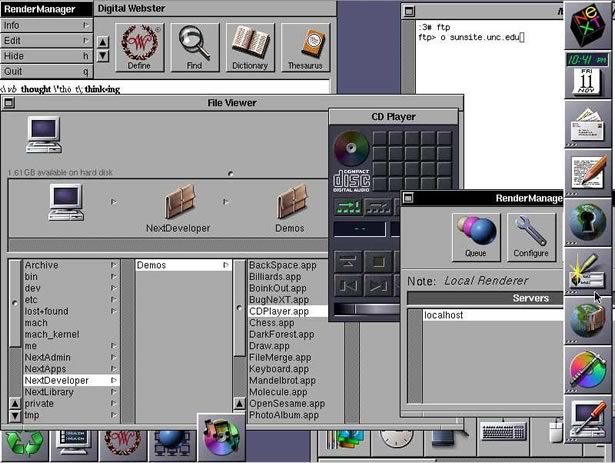
\includegraphics[width=0.4\textwidth]{figs/nextstep.jpg}

(1) DOS '81
(2) Classic '84
(3) Window 3.1 '92
(4) OpenStep '89
\end{frame}

\end{document}
